\section{Related Work}
\label{section:relatedwork}
Out method facilitates local data analysis in linear projections. We adopt the strategy of projection pursuit to find desirable projections, as opposed to dimension-driven exploration methods. We'll briefly introduce related works in the relevant fields.

\subsection{Data Locality Analysis in Projections}
Data locality has been extensively studied in high-dimensional data researches. There are roughly two branches, focusing on different aspects.

The major branch aims to improve global projections, focusing on preserving data localities. Lots of non-linear projections have been proposed for this purpose, such as Laplacian Eigenmaps (LE)~\cite{DBLP:journals/neco/BelkinN03}, Locally Linear Embedding (LLE)~\cite{roweis2000nonlinear}, Local Tangent Space Alignment (LTSA)~\cite{DBLP:journals/corr/cs-LG-0212008}, etc. These methods fit for data lying on a low-dimensional manifold (e.g. images of faces). But the semantics of dimensions are weakened or lost. Users cannot know in which dimensions the data are similar or different. Hence, these methods are not suitable for general high-dimensional data with meaningful dimensions. In comparison, our method keeps all projections in a linear framework. It helps to explain data relationships in the context of dimensions.

Another branch aims to reveal distortions in a projection. Martins et al.~\cite{DBLP:journals/cg/MartinsCMT14} examined distortions in different types of projections. They used color mapping to indicate distortion levels, and helped find real neighborhoods with automatic algorithms. Liu et al. took a step~\cite{DBLP:journals/cgf/LiuWBP14} further by analyzing data structures based on distortions. But none of them provide means to correct the distorted relationships. Stahnke et al.~\cite{DBLP:journals/tvcg/StahnkeDMT16} proposed a simple correction by directly changing point distances. However, such method is too straightforward to support a more in-depth local analysis. In this work, we also offer to show and correct distance distortions. But the correction here is achieved by changing the whole projection. It can reduce distortions for a small neighborhood rather than a single datum.

\begin{figure*}[htbp]
\centering
  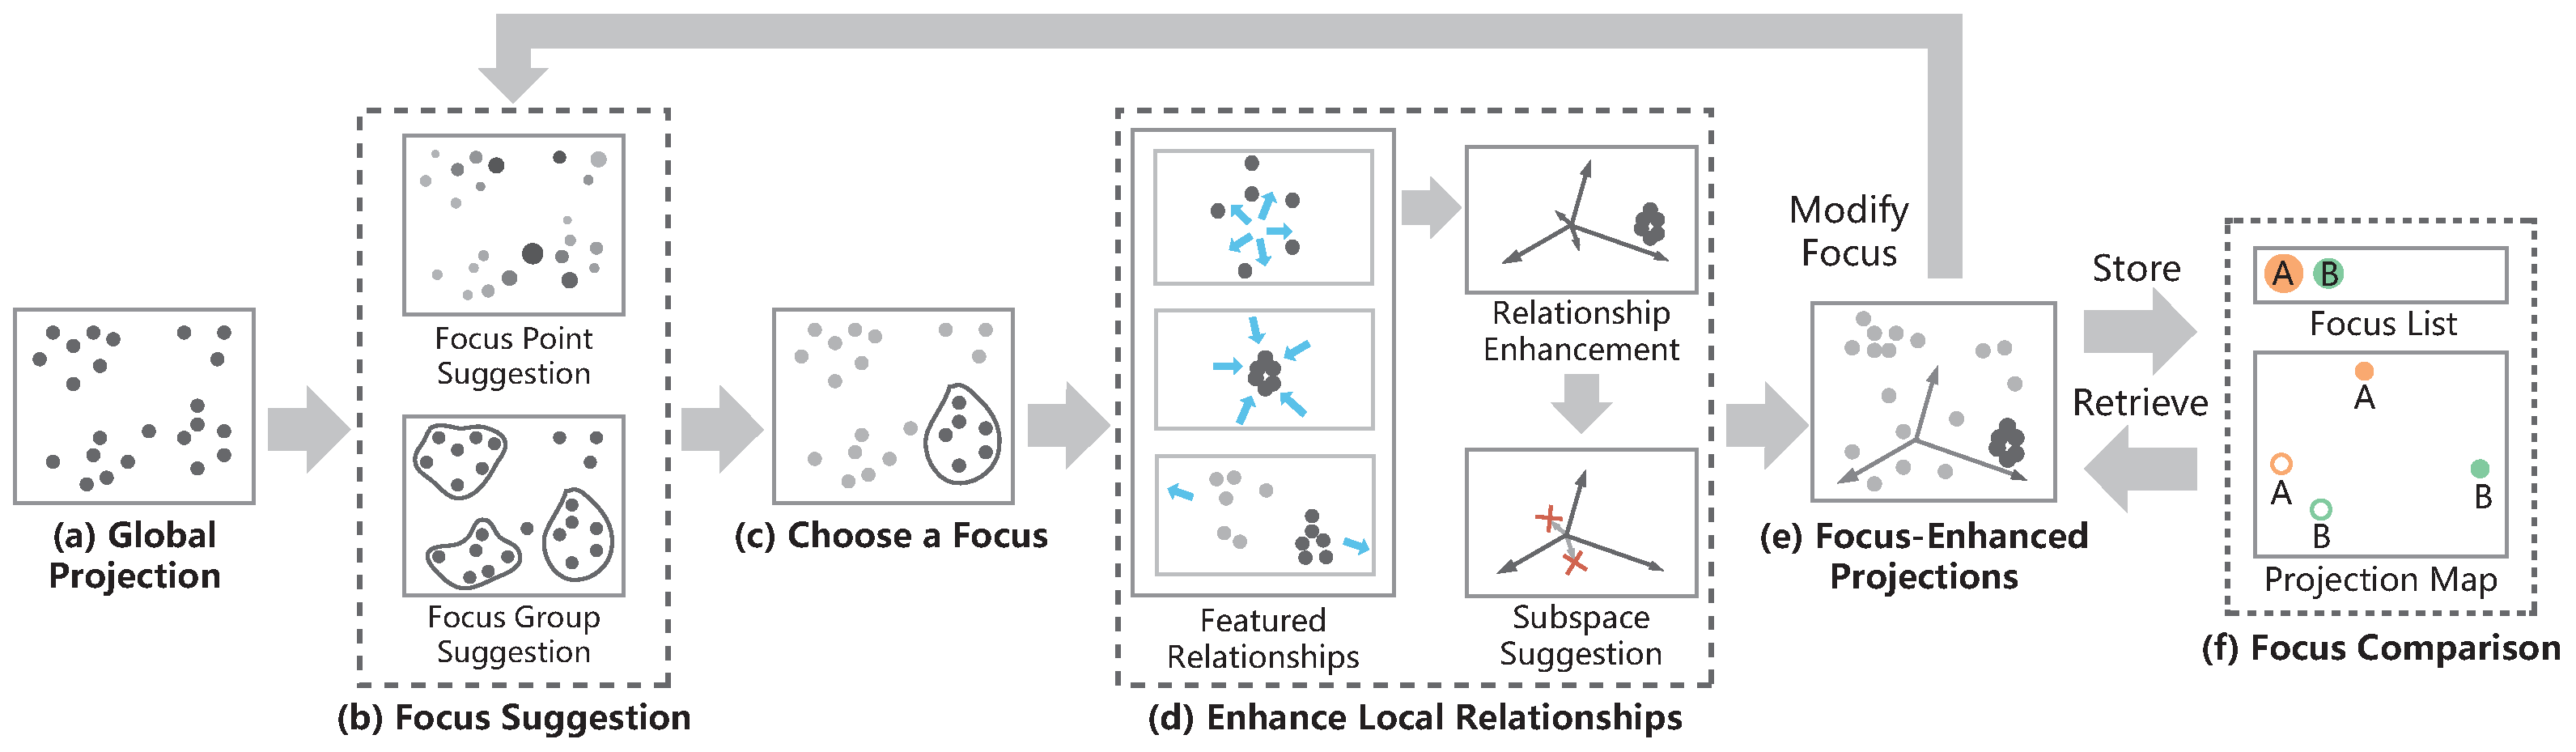
\includegraphics[width=1\linewidth]{images/new_pipeline.eps}% 1\linewidth
  \caption{Overview of the proposed exploration process.}
\label{fig:workflow}
  \end{figure*}

\subsection{Projection Assisted Data Exploration}
Dimension reduced projections are often used to explore high-dimensional data. They are intuitive overviews, but hard to be changed interactively. Jeong et al.~\cite{DBLP:journals/cgf/JeongZFRC09} allow users to change a projection by updating dimension weights in the PCA algorithm. Nam et al.~\cite{DBLP:journals/tvcg/NamM13} took a step further. They let users directly decide dimension components in a projection. Beyond parameter tuning, Lehmann et al.~\cite{DBLP:journals/tvcg/LehmannT13} proposed a more intuitive interaction. Users can alter the dimension axes while maintaining an orthogonal mapping. These methods are indeed effective. But users have to go through an exhausting trial-and-error process, since they cannot foresee the effects of dimension changes. Our method allows users to specify local data and relationships, rather than dimension weights. It's more intuitive and more efficient. Users don't have to search by themselves, but can still get insightful projections.

In a projection assisted exploration, subspace clusters are often provided beforehand~\cite{DBLP:conf/ieeevast/TatuMFBSSK12}~\cite{DBLP:journals/tvcg/NamM13}~\cite{DBLP:journals/cgf/LiuWTBP15}. In some other methods~\cite{DBLP:journals/tois/ChenL06}~\cite{DBLP:conf/ieeevast/NamHMZI07}~\cite{DBLP:conf/ieeevast/TatuMFBSSK12}, users are able to participate in the automatic clustering process. But in either way, users don't fully understand the given clusters or subspaces. It's hard for them to modify the results, let alone discovering more hidden clusters. Yuan et al.~\cite{DBLP:journals/tvcg/YuanRWG13} proposed a hierarchical subspace exploration, which is the most relevant to our method. They allow users to analyze a local subset in different subspaces. It helps to discover hidden local clusters. However, they did not provide any guidance for subspace selection. Besides, the lack of data context makes it hard to comprehend and modify the local subset.
\note{
	\textbf{Subspace Cluster Estimation}
	\note{~\cite{DBLP:journals/tsp/CarterRH10}}%Intrinsic Dimension
	~\cite{DBLP:conf/ieeevast/Kandogan12}%Just-in Time
	~\cite{DBLP:journals/tvcg/YuanRWG13}%Subspace Cluster
}

\subsection{Feature Driven Projection Selection}
Projection pursuit~\cite{DBLP:journals/tc/FriedmanT74}~\cite{cook1995grand} is a well-known technique for finding interesting projections. It generates a series of projections to optimize a certain index. Gleicher et al.~\cite{DBLP:journals/tvcg/Gleicher13} used machine learning to train compositive dimensions for classification. Choo et al.~\cite{DBLP:conf/ieeevast/ChooLKP10} made the process interactive by involving users in a semi-supervised Linear Discriminant Analysis (LDA). In both works, user-defined classes are imported as the pursuit index. Apart from the classes, user-defined layouts can also act as the target~\cite{DBLP:journals/tvcg/JoiaCCPN11}~\cite{DBLP:conf/ieeevast/BrownLBC12}~\cite{DBLP:journals/tvcg/HuBMHNL13}. However, these methods require the user to have solid prior knowledge, which is often not the case in a data exploration.

The rank-by-feature framework~\cite{DBLP:journals/ivs/SeoS05} is a variant of projection pursuit. It ranks existing projections according to feature strengths. Various kinds of metrics~\cite{DBLP:conf/ieeevast/AlbuquerqueEM11} are defined to measure different features, including class separation~\cite{DBLP:journals/cgf/SipsNLH09}~\cite{DBLP:journals/cgf/SedlmairTMT12}, clustering / outliering~\cite{DBLP:conf/ieeevast/TatuAESTMK09}~\cite{DBLP:journals/tvcg/JohanssonJ09}, and more complex topological properties~\cite{DBLP:conf/infovis/WilkinsonAG05}. They are helpful for analyzing a large group of scatterplots~\cite{DBLP:conf/apvis/NhonW14}~\cite{DBLP:conf/ieeevast/AnandWN12}. But most of them are result-oriented. Some measurements even depend on the display space. It's hard to use them to guide the generation of projection. Besides, they are too complex to compute. The time spent to find and score a projection will be unbearable in an interactive exploration. For these reasons, we only consider simple metrics, when using the strategy of projection pursuit to get desirable projections. The simple criteria are not only more efficient, but also easier to interpret.
\note{
~\cite{DBLP:conf/infovis/WilkinsonAG05}%Scagnostics
~\cite{DBLP:conf/ieeevast/AlbuquerqueEM11}%quality measures
~\cite{DBLP:conf/ieeevast/TatuAESTMK09}%combining automatic analysis
~\cite{DBLP:journals/cgf/SipsNLH09}%class consistency
~\cite{DBLP:journals/cgf/SedlmairTMT12}%class separation
~\cite{DBLP:journals/tvcg/JohanssonJ09}%combination of metrics
~\cite{DBLP:conf/apvis/NhonW14}%scagexplorer
~\cite{DBLP:conf/ieeevast/AnandWN12}%random projection

\textbf{Projection Pursuit for Classification}
~\cite{DBLP:conf/ieeevast/ChooLKP10}%iVisClassifier

\textbf{Targeted Projection Pursuit}
}